\section{Lezione del 9 novembre}
\subsection{Bisimulazione debole}

Una relazione $R\subseteq Proc_{CCS}\times Proc_{CCS}$ è una bisimulazione debole $\iff \forall p,q \in Proc_{CCS} \; | \; pRq$, vale che $\forall a\in Act = A \cup \bar{A} \cup \{\tau\}$,
\begin{itemize}
    \item se $p\stackrel{a}{\rightarrow}p_1$, allora esiste $q\stackrel{a}{\Rightarrow}q_1$ tale che $p_1Rq_1$
    \item se $q\stackrel{a}{\rightarrow}q_1$, allora esiste $p\stackrel{a}{\Rightarrow}p_1$ tale che $p_1Rq_1$
\end{itemize}

Quindi due processi $p$ e $q$ sono in \textbf{bisimulazione debole} $(p\stackrel{bis}{\approx}q) \iff \exists$ una relazione di bisimulazione $R$ tale che $pRq$. E quindi la relazione di bisimulazione è corrispondente a:
$$\stackrel{Bis}{\approx} =\bigcup\{R \; | \; R\textnormal{ è di bisimulazione debole} \}$$

\subsection{Bisimulazione debole come gioco} 
Regole del gioco che spiegano come capire se due processi sono bisimili. Per confrontare due processi CCS, $p$ e $q$, è possibile usare un gioco $G(p,q)$ con due giocatori, quali:
\begin{enumerate}
    \item attaccante: cerca di dimostrare $p\stackrel{Bis}{\not\approx}q$
    \item difensore: cerca di dimostrare $p\stackrel{Bis}{\approx}q$
\end{enumerate}
Un gioco è costituito da più partite, ognuna delle quali consiste in una sequenza finita o infinita di configurazioni o \textit{mani} $(p_0,q_0), \dots, (p_i,q_i) \dots$.
In ogni mano si passa dalla configurazione corrente a quella successiva tramite diverse regole:
\begin{itemize}
    \item l’attaccante sceglie uno dei processi della configurazione corrente $(p_i,q_i)$ e fa una $\stackrel{a}{\rightarrow}$ mossa ($a \in Act)$ con la regola forte.
    \item il difensore deve rispondere con una \textit{mossa} $\stackrel{a}{\Rightarrow}$ con la regola debole, sull’altro processo.
\end{itemize}
La nuova coppia $(p_{i+1},q_{i+1})$ ottenuta in questo modo diventa la nuova configurazione corrente e la partita continua con l’altra mano. Se un giocatore non può più muovere l’altro vince; inoltre se la partita è infinita vince il difensore.
Diverse partire possono concludersi con vincitori diversi ma per ogni gioco un solo giocatore può vincere la partita. 

Una \textbf{strategia} per un giocatore è un insieme di regole che indicano di volta in volta che mossa fare e che dipendono solo dalla configurazione corrente.\\
Diciamo che un giocatore ha una \textbf{strategia vincete} se per $G(p,q)$, seguendo quella strategia, vince tutte le partite del gioco.
\begin{teorema}{Teorema}{}
    \par\centering
    Per ogni gioco $G(p,q)$ solo uno dei due giocatori ha una strategia vincente.
\end{teorema}
\begin{teorema}{Teorema}{}
    \par\centering
    L’attaccante ha una strategia vincente $\iff p \stackrel{Bis}{\not\approx}q$.\\
    Il difensore ha una strategia vincente $\iff p \stackrel{Bis}{\approx}q$.
\end{teorema}

A questo punto il gioco della bisimulazione può essere usato sia per dimostrare che due processi sono bisimili, sia per dimostrare che non lo sono:
\begin{itemize}
    \item per dimostrare che sono bisimili, bisogna mostrare che per ogni mossa dell’attaccante il difensore ha almeno una mossa che lo porterà a vincere.
    \item per vedere che non sono bisimili, bisogna dimostrare che in ogni configurazione l’attaccante è in grado di scegliere su quale processo operare e con quale azione, in modo tale che per ogni risposta del difensore l’attaccante avrà almeno una mossa che lo porterà a vincere.
\end{itemize}
\subsubsection{Esempio chiarificatore}
Vediamo l'esempio di un gioco con due processi che dimostreremo essere bisimili:\\
Siano:
\begin{itemize}
    \item $p_1=a\cdot(b\cdot Nil+\tau\cdot c\cdot Nil)$ (sinistra)
    \item $u_1=a\cdot(b\cdot Nil+\tau\cdot c\cdot Nil)+a\cdot c\cdot Nil$ (destra)
\end{itemize}
\begin{figure}[H]
    \centering
    \begin{minipage}[b]{.35\textwidth}
        \centering
        \begin{tikzpicture}[shorten >=1pt,node distance=2cm,on grid,auto] 
          \node[state] (q_0) {$q_1$};  
          \node[state] (q_1) [below left =of q_0] {$q_2$};
          \node[state] (q_2) [below right =of q_0] {$q_3$};
          \node[state] (q_3) [below right =of q_1] {$Nil$};
          \path[->]
          (q_0) edge [above left] node {$a$} (q_1)
          (q_0) edge  node {$a$} (q_2)
          (q_1) edge [below left] node {$b$} (q_3)
          (q_2) edge  node {$c$} (q_3)
          ;
        \end{tikzpicture}
        \caption{$p_1$}
        \label{fig:prob1_6_2}
    \end{minipage}%
    \begin{minipage}[b]{0.35\textwidth}
        \centering
        \begin{tikzpicture}[shorten >=1pt,node distance=2cm,on grid,auto] 
            \node[state] (q_0) {$u_1$};  
            \node[state] (q_1) [below= of q_0] {$u_2$};
            \node[state] (q_2) [left = of q_1] {$u_3$};
            \node[state] (q_3) [right  =of q_1] {$u_4$};
            \node[state] (q_4) [below =of q_1] {$Nil$};
            \path[->]
            (q_0) edge [above left] node {$a$} (q_1)
            (q_0) edge  node {$a$} (q_3)
            (q_1) edge  node {$b$} (q_4)
            (q_1) edge  node {$\tau$} (q_2)
            (q_2) edge [below left] node {$c$} (q_4)
            (q_3) edge [below right] node {$c$} (q_4)
            ;
        \end{tikzpicture}
        \caption{$u_1$}
        \label{fig:prob1_6_1}
    \end{minipage}
\end{figure}
Vediamo quindi come si svolgono tutte le partite per $G(p_1,u_1)$:
\begin{itemize}
    \item all'inizio l'attaccante può fare $p_1\stackrel{a}{\rightarrow}p_2$ e il difensore può fare $u_1\stackrel{a}{\Rightarrow}u_2$, ed è la scelta vincente, avendo che $p_2$ e $u_2$ sono isomorfi. Una scelta buona su tre possibilità
    \item all'inizio l'attaccate può fare $u_1\stackrel{a}{\rightarrow}u_2$ e il difensore può fare $p_1\stackrel{a}{\Rightarrow}p_2$, ed è la scelta vincente, avendo che $p_2$ e $u_2$ sono isomorfi. Una scelta buona su due possibilità
    \item all'inizio l'attaccate può fare $u_1\stackrel{a}{\rightarrow}u_4$ e il difensore può fare $p_1\stackrel{a}{\Rightarrow}p_3$, ed è la scelta vincente, avendo che $p_3$ e $u_4$ sono isomorfi.Una scelta buona su tre possibilità
\end{itemize}
Il difensore ha quindi una strategia vincente.
Ho quindi che la relazione di bisimilitudine: $R=\{(p_1,u_1),(p_2,u_2),(p_3,u_3),(p_3,u_4),(Nil,Nil)\}$, e quindi: $p_1\stackrel{Bis}{\approx}u_1$ . \\
Posso fare una rappresentazione ad albero, che vediamo in modo parziale, segnando in verde le mosse vincenti dei difensori (con processi bisimili):
\begin{center}
    \begin{tikzpicture}
    \tikzstyle{bplus}=[rectangle split, rectangle split horizontal,rectangle split ignore empty parts,draw]
    \tikzstyle{every node}=[bplus]
    \tikzstyle{level 1}=[sibling distance=45mm]
    \tikzstyle{level 2}=[sibling distance=15mm]
    \node {$p_1,\ u_1$} [->]
      child {node {$p_2,\ u_1$ }
        child[draw=green,thick] {node[draw=blue!80, thick]{$p_2,\ u_2$}}
        child {node {$p_2,\ u_3$}}
        child {node {$p_2,\ u_4$}}    
      } 
      child {node {$p_1,\ k_2$ }
        child[draw=green,thick] {node[draw=blue!80, thick]{$p_2,\ u_2$}}
        child {node {$p_3,\ u_2$}}
      } 
      child {node {$p_1,\ u_4$ }
        child {node{$p_2,\ u_4$}}
        child[draw=green,thick] {node[draw=blue!80, thick] {$p_3,\ u_4$}}
      } 
    ;\end{tikzpicture}
\end{center}

\subsection{Secondo esempio}
Vediamo l'esempio di un gioco con due processi che dimostreremo non essere  bisimili, siano quindi:
\begin{itemize}
    \item $q_1=a\cdot b\cdot Nil+a\cdot c\cdot Nil$, nella figura a sinistra
    \item $u_1=a\cdot (\tau\cdot b\cdot Nil+\tau\cdot c\cdot Nil)$, in quella a destra
\end{itemize}
Abbiamo quindi:
\begin{figure}[H]
    \centering
    \begin{minipage}[b]{.35\textwidth}
        \centering
        \begin{tikzpicture}[shorten >=1pt,node distance=2cm,on grid,auto] 
          \node[state] (q_0) {$q_1$};  
          \node[state] (q_1) [below left =of q_0] {$q_2$};
          \node[state] (q_2) [below right =of q_0] {$q_3$};
          \node[state] (q_3) [below right =of q_1] {$Nil$};
          \path[->]
          (q_0) edge [above left] node {$a$} (q_1)
          (q_0) edge  node {$a$} (q_2)
          (q_1) edge [below left] node {$b$} (q_3)
          (q_2) edge  node {$c$} (q_3)
          ;
        \end{tikzpicture}
        \caption{$q_1$}
    \end{minipage}%
    \begin{minipage}[b]{0.35\textwidth}
        \centering
        \begin{tikzpicture}[shorten >=1pt,node distance=2cm,on grid,auto]
          \node[state] (q_0) {$u_2$};  
          \node[state] (q_1) [below left =of q_0] {$u_3$};
          \node[state] (q_2) [below right =of q_0] {$u_4$};
          \node[state] (q_3) [below right =of q_1] {$Nil$};
          \node[state] (q_4)[above =of q_0]  {$u_1$}; 
          \path[->]
          (q_0) edge [above left] node {$\tau$} (q_1)
          (q_0) edge  node {$\tau$} (q_2)
          (q_1) edge [below left] node {$b$} (q_3)
          (q_2) edge  node {$c$} (q_3)
          (q_4) edge  node {$a$} (q_0)
          ;
        \end{tikzpicture}
        \caption{$u_1$}
    \end{minipage}
\end{figure}
Vediamo quindi come si svolgono tutte le partite per $G(q_1,u_1)$.\\ 
L'attaccante esegue $u_1\stackrel{a}{\rightarrow}u_2$.Nella situazione attuale il difensore ha due scelte:
\begin{itemize}
    \item $q_1\stackrel{a}{\Rightarrow}q_2$. Sono quindi in $(q_2,u_2)$. A questo punto $u_2\stackrel{\tau}{\rightarrow}u_4$ a cui il difensore non può che rispondere con l’azione nulla, $q_2\stackrel{\tau}{\rightarrow}q_2$, perdendo in quanto $q_2\stackrel{Bis}{\not\approx} u_4$ dato che dal primo, $q_2$ posso fare solo $b$ e dal secondo, $u_4$ solo $c$
    \item $q_1\stackrel{a}{\Rightarrow}q_3$. Sono quindi in $(q_3,u_2)$. A questo punto $u_2\stackrel{\tau}{\rightarrow}u_3$ a cui il difensore non può che rispondere con l’azione nulla, $q_3\stackrel{\tau}{\rightarrow}q_3$, perdendo in quanto $q_3\stackrel{Bis}{\not\approx} u_3$ dato che dal primo, $q_3$, posso fare solo $c$ e dal secondo, $u_3$, solo $b$
  \end{itemize}
Quindi abbiamo fatto vedere, con un esempio, che ci sono dei casi di non bisimilutidine: $q_1\stackrel{Bis}{\not\approx} u_1$\\
Vediamo anche in questo caso un albero parziale, dove si vedono anche le mosse in cui l'attaccante perdeva. Sono di egual colore le configurazioni identiche e si hanno col bordo con spessore più grande le foglie (non colorate) corrispondi alle vincite del difensore, che però non ha sempre una mossa per risponde attaccante, comportando la non bisimulazione:
Le foglie colorate rappresentano parti di alberi parziali.
\begin{figure}[H]
    \centering
    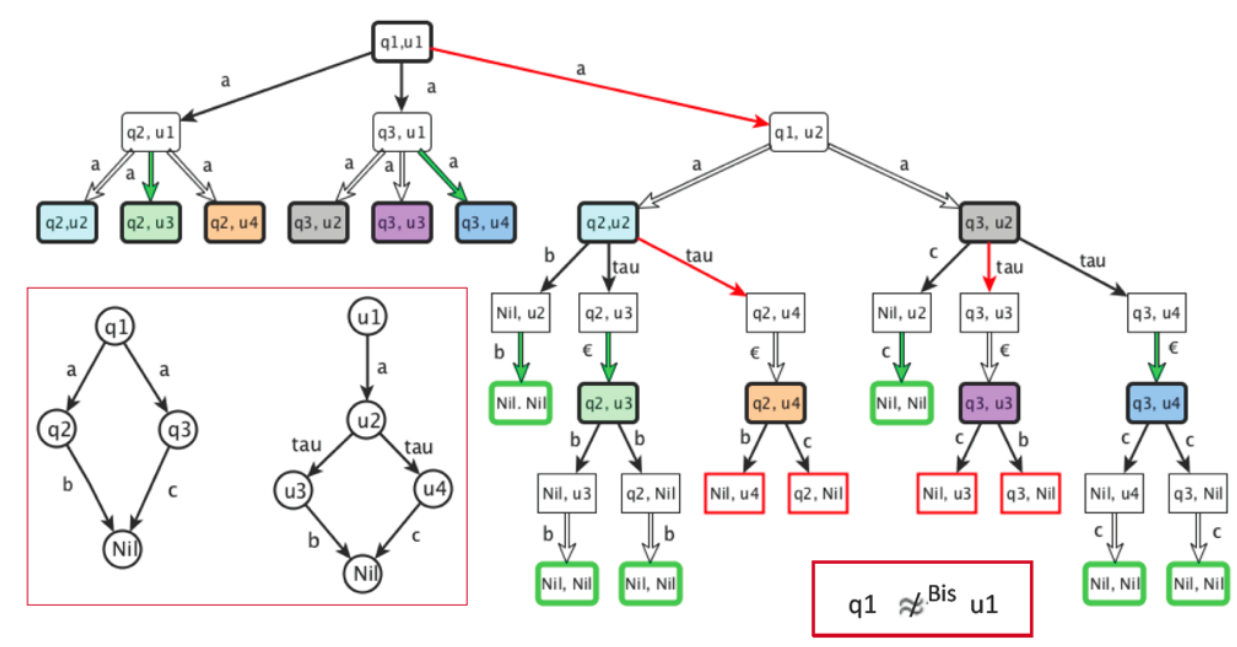
\includegraphics[scale = 0.4]{IMM/albero_grosso.PNG}
\end{figure}